% !TEX root = ../../report.tex

\subsection{PCB Workarounds}

Due to the manual work involved in designing the PCB, and because it was fairly
unfamiliar ground for everyone involved, there were many things that could go
wrong. This section describes everything that was wrong with the PCB along with
what was done to fix it.

The first thing to happen was smoke appearing from the linear regulator upon
plugging in the power source. As it turned out, the footprint was mismatched
with the pinout of the component. The footprint had been fixed early on in the
process, but unfortunately the schematics had not been updated. The same turned
out to have happened with the low frequency crystal connected to the MCU,
although this component did not produce any smoke.

Both of the above problems where solved by extra wiring. For the crystal, where
pin 1 and 4 was suppose to be used, pin 1 and 2 were used instead. As pins 2 and
3 were unconnected, a patch cable was soldered between pin 4 and 2.

\begin{figure}[H]
    \centering
    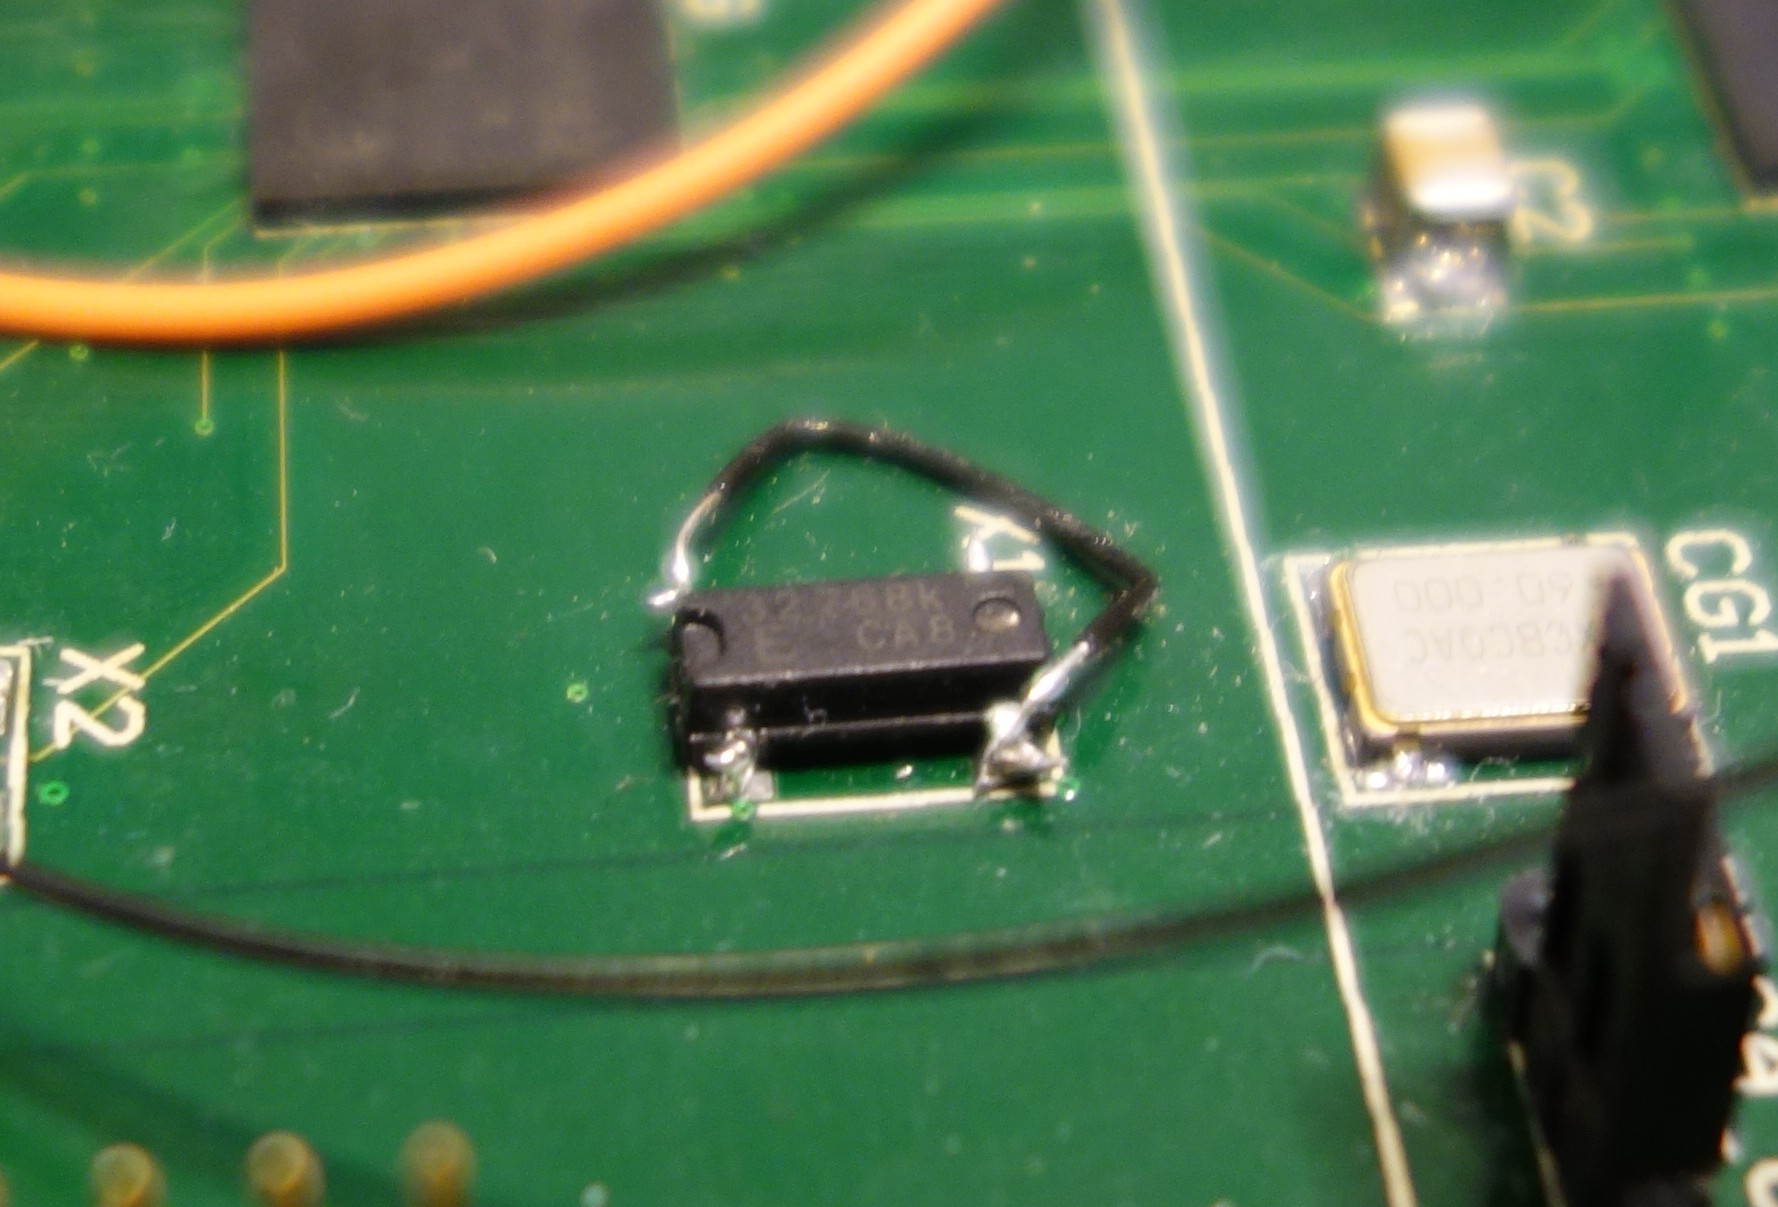
\includegraphics[scale=0.1]{figures/results/pcb/lfxtal}
    \caption{Low frequency crystal hack.}
    \label{fig:res:lfxtal}
\end{figure}



The linear regulator was slightly more advanced as pin 1 and 5, and 2, 3 and 4,
had been swapped. The solution was to solder six short patch cables on the pads
themselves, and then match the feet of the linear regulator with the right
cables. This resulted in the linear regulator being mounted about 1 cm above the
card.

\begin{figure}[H]
    \centering
    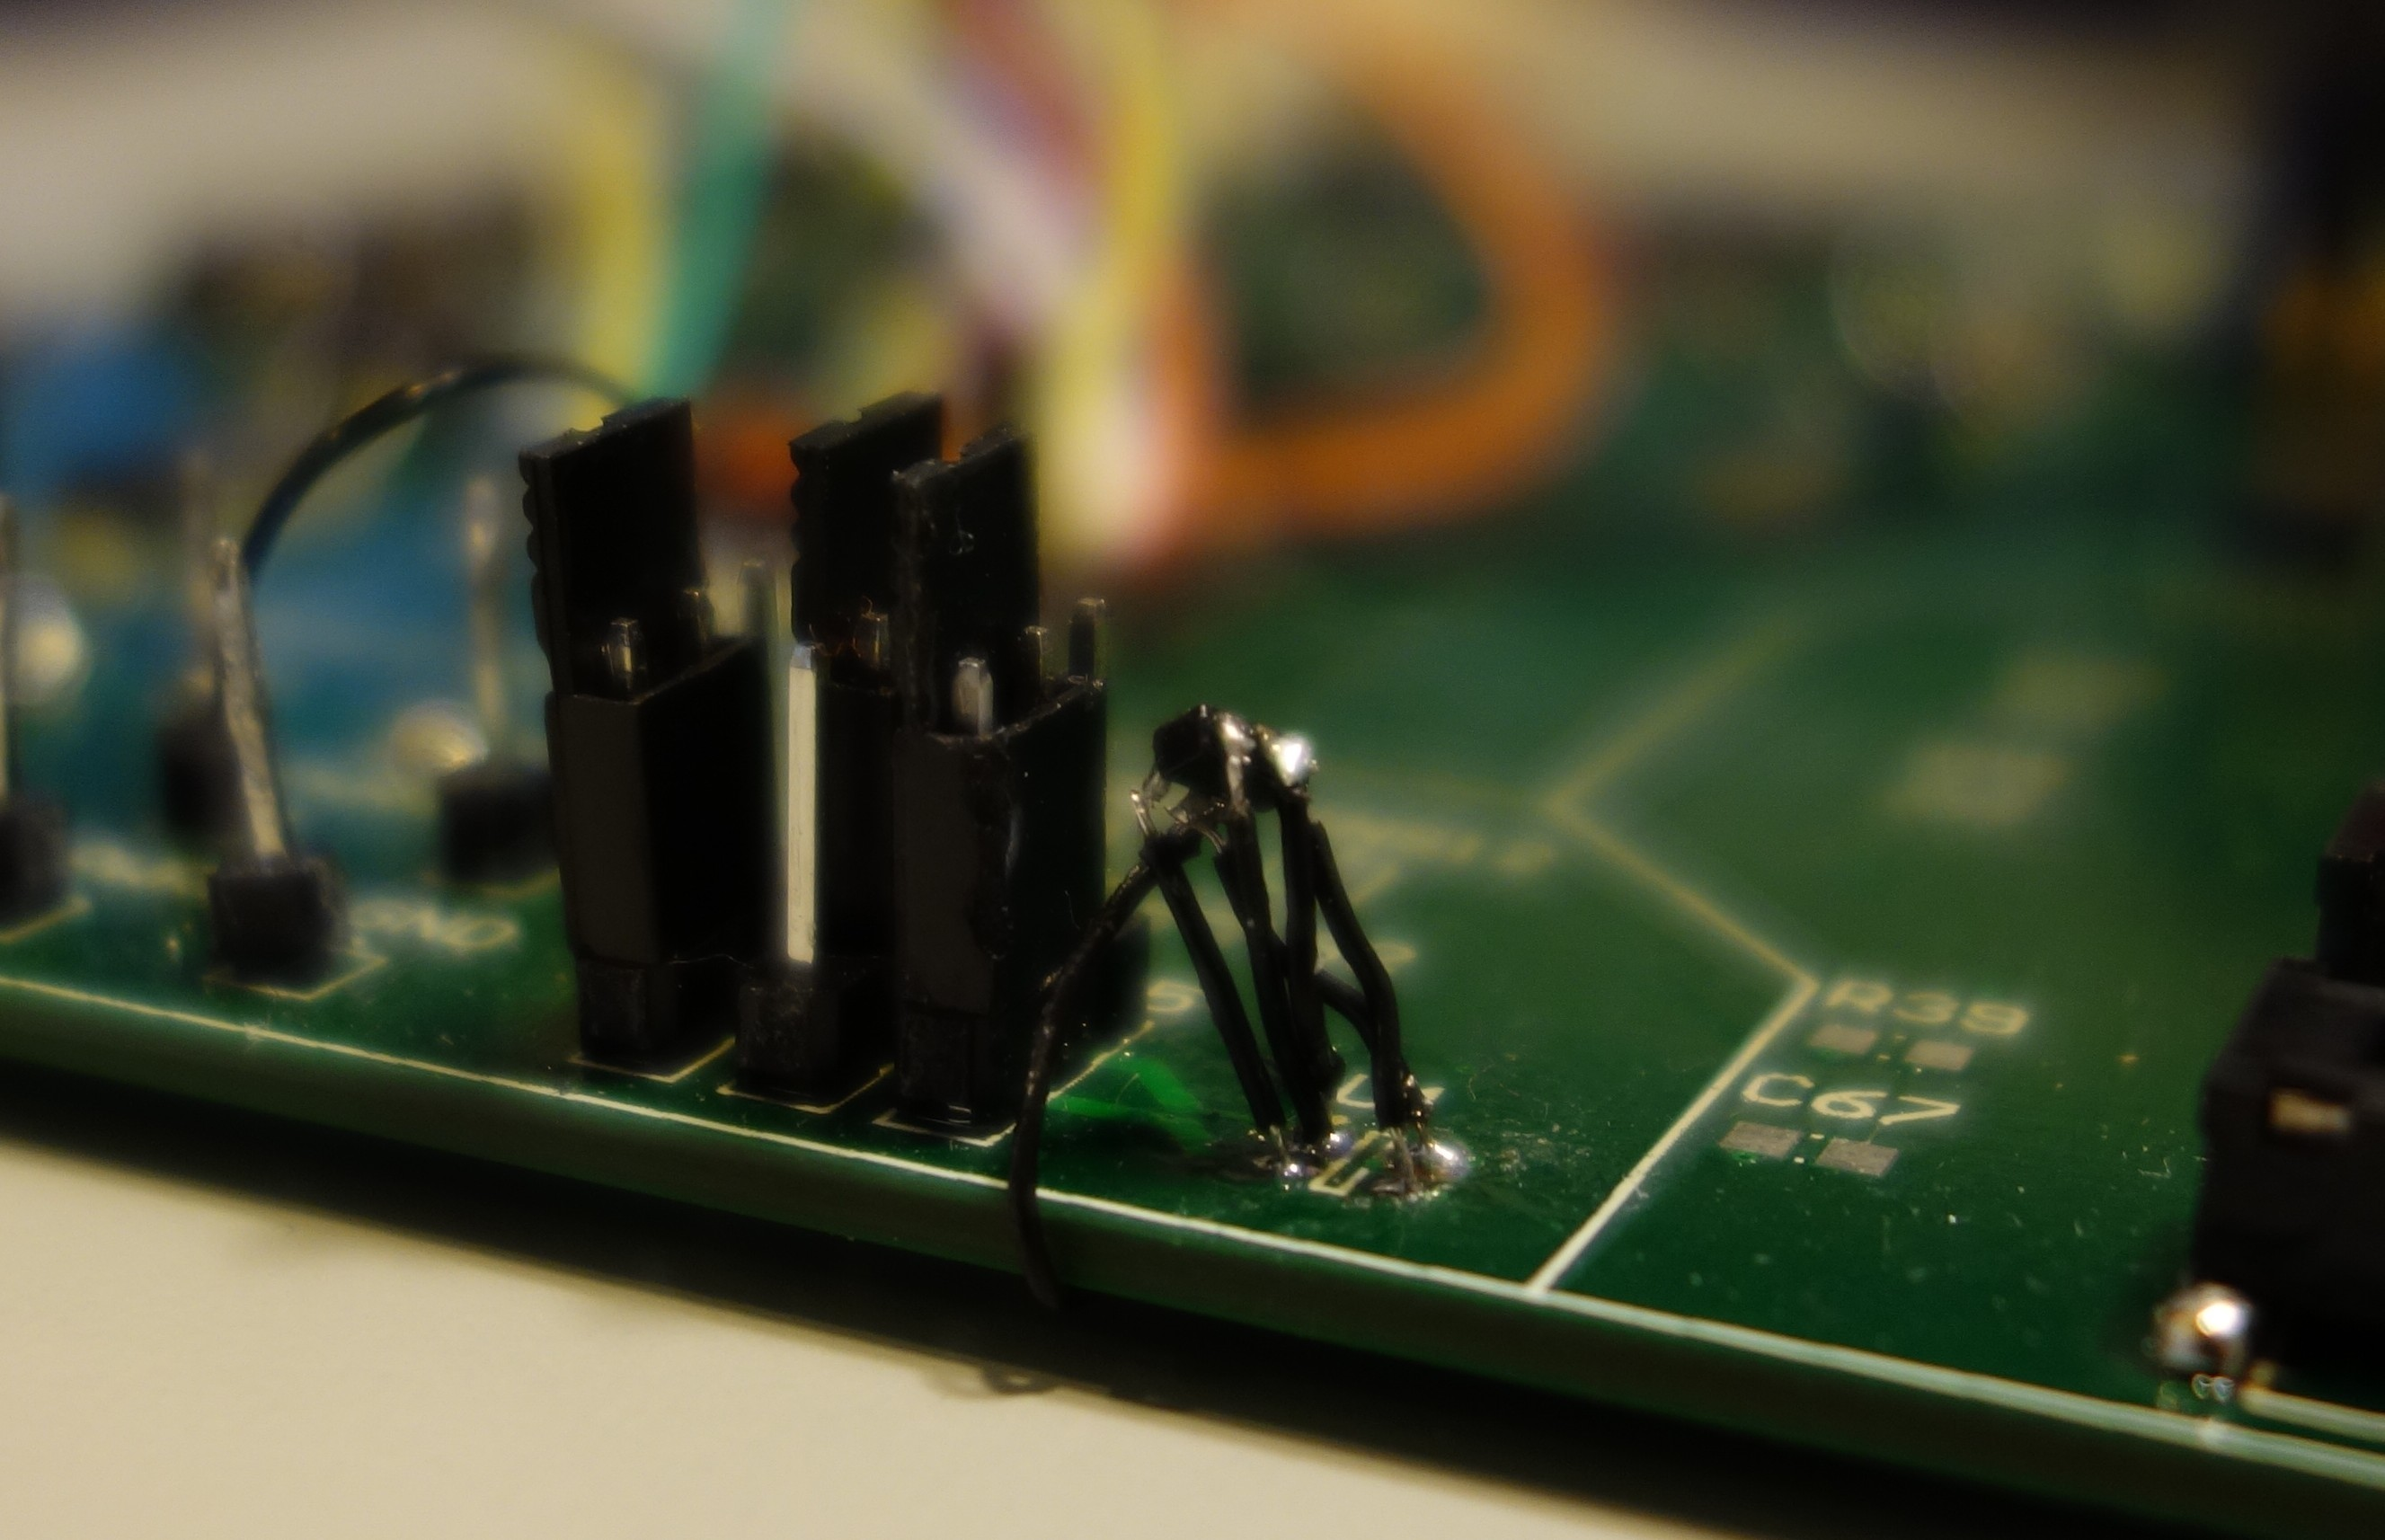
\includegraphics[scale=0.1]{figures/results/pcb/linear-regulator.jpg}
    \caption{Linear voltage regulator hack.}
    \label{fig:res:linreg}
\end{figure}



In addition, due to a typo in the schematic, the data lines of the EBI bus were
only connected to the MCU and external RAM, not to the FPGA. Again, this was
solved by patch cables between the external RAM's data pins and all available
FPGA GPIO pins. The result was a fully functional bus as was originally
intended, at the expense of all other I/O opportunities on the FPGA. All 12 GPIO
pins were used, as well as two buttons and two LED's, adding up to 16 bits.

% !TEX root = ../../../../report.tex
\subsubsection{Bus interface}

While not strictly a component, the databus is still an important part of
the PCB design. The MCU natively supports two bus interfaces, I2C and EBI,
of which the latter was used. This was done because I2C as a
serial bus has more limited bandwidth compared to the EBI, which
supports 16 bit words. The need for speed stems from the requirement of
streaming at least two audio streams live between the MCU and FPGA.
As an added bonus, the EBI bus is compatible with SRAM chip interfaces
which proved useful when including extra memory in the design.

In addition to the EBI bus there is a special control bus with a width
of 3 signals going between the MCU and FPGA. This bus is available for the
software and FPGA group to use as needed, for instance for interrupts or
other forms of synchronization and status signaling.


Finally, there was an actual connection error in the external RAM footprint.
One of the two chip select inputs, CS1, was suppose to be grounded, but had
mistakenly been connected to VCC33, resulting in the unit being stuck in off
mode. To solve this, the chip select pin was bent slightly upwards and then
connected with a patch cable to a GND pin nearby. However, due to the bus
workaround the SRAM was completely disabled and not used.

